According to \cite{TheAdaptiveWeb} there are seven, most commonly used implementations of hybrid recommendation systems. These implementations can be split into 3 groups.

\begin{itemize}
\item Weighted
\item Switching
\item Mixed
\item Feature combination
\item Feature augmentation
\item Cascade
\item Meta-level
\end{itemize}

The weighted, switching, and mixed solutions all produce individual recommendations the same way a single non-hybrid system would. The candidates are then worked in some way before the resulting recommendations are found.

The second group consists of the feature combination and feature augmentation which through mixing the logic of the different recommendation systems makes it possible for a recommender to have another source than what it was originally made for. These are especially good when the original source is inadequate for the job and you need other sources to draw from.

The last group consists of the cascade and the meta-level hybrids. They specialize by working in succession thereby strengthening each other's candidates. This can be a good way to get a higher precision if the first recommender ties a score on several items. Then the second recommender can do further work on them. 

\subsubsection{Weighted, switching and mixed hybrids} 
We chose to look closer at the first group of hybrids as we came to the conclusion that these were within our capabilities and would satisfy our needs when recommending media.



\textbf{The weighted hybrid}


\begin{figure}[H]
\centering
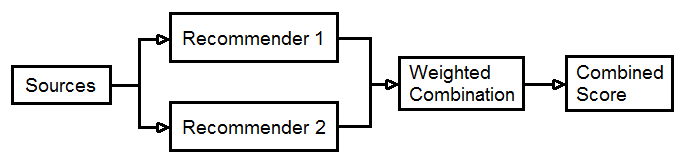
\includegraphics[width=0.8\textwidth]{Images/Weightedhybrid.png}
\caption{Weighted hybrid}
\label{Weighted}
\end{figure}
As shown in \ref{Weighted} the weighted hybrid works by letting each recommender attach a score to their candidates and the candidates combined score is calculated. The top scoring candidates are then presented to the user. 



\textbf{The mixed hybrid}


\begin{figure}[H]
\centering
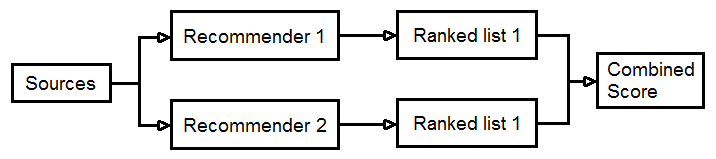
\includegraphics[width=0.8\textwidth]{Images/Mixedhybrid.png}
\caption{Mixed hybrid}
\label{Mixed}
\end{figure}
As shown in \ref{Mixed} the mixed hybrid combines the candidates from each recommender into pairs and presents them to the user without trying to work the results further.



\textbf{The switching hybrid}


\begin{figure}[H]
\centering
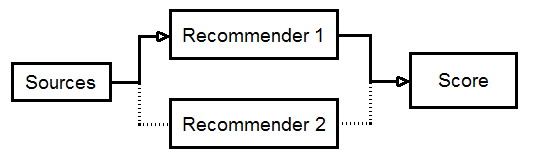
\includegraphics[width=0.8\textwidth]{Images/Switchinghybrid.png}
\caption{Switching hybrid}
\label{Switching}
\end{figure}
As shown in \ref{Switching}, this hybrid works by using the best recommender for the situation. If recommender 1 gives the best results for one user that recommender is used. For another user recommender 2 might be more precise and is therefore used instead for that user.
